\documentclass[10pt,executivepaper]{article}
\usepackage[utf8]{inputenc}
\usepackage[spanish]{babel}
\usepackage{amsmath}
\usepackage{amsfonts}
\usepackage{amssymb}
\usepackage{graphics}
\usepackage{graphicx}
\usepackage[left=2cm,right=2cm,top=2cm,bottom=2cm]{geometry}
\usepackage{imakeidx}
\makeindex[columns=3, title=Alphabetical Index, intoc]
\usepackage{listings}
\usepackage{xcolor}
\usepackage{multicol}
\usepackage{changepage}
\usepackage{float}
\usepackage{cite}
\usepackage{url}
\usepackage{pdflscape}

\definecolor{codegreen}{rgb}{0,0.6,0}
\definecolor{codegray}{rgb}{0.5,0.5,0.5}
\definecolor{codepurple}{rgb}{0.58,0,0.82}
\definecolor{backcolour}{rgb}{0.95,0.95,0.92}

\lstdefinestyle{mystyle}{
    backgroundcolor=\color{backcolour},
    commentstyle=\color{codegreen},
    keywordstyle=\color{magenta},
    numberstyle=\tiny\color{codegray},
    stringstyle=\color{codepurple},
    basicstyle=\ttfamily\footnotesize,
    breakatwhitespace=false,
    breaklines=true,
    captionpos=b,
    keepspaces=true,
    numbers=left,
    numbersep=5pt,
    showspaces=false,
    showstringspaces=false,
    showtabs=false,
    tabsize=3
}

\def\fillandplacepagenumber{%
 \par\pagestyle{empty}%
 \vbox to 0pt{\vss}\vfill
 \vbox to 0pt{\baselineskip0pt
   \hbox to\linewidth{\hss}%
   \baselineskip\footskip
   \hbox to\linewidth{%
     \hfil\thepage\hfil}\vss}}


\lstset{style=mystyle}

\title{Actividad: Implementación de un token-ring}

\author{Instituto Politécnico Nacional\\Escuela Superior de Computo\\Desarrollo de Sistemas Distribuidos\\Adrian González Pardo\\4CV1\\21/01}
\date{\today}
\newcommand\tab[1][1cm]{\hspace*{#1}}

\begin{document}
\maketitle
\section{Código fuente:}
\begin{center}
  \lstinputlisting[language=Java]{../Token.java}
  \lstinputlisting[language=Bash]{../Makefile}
\end{center}
\section{Capturas y descripción del programa}
\begin{center}
  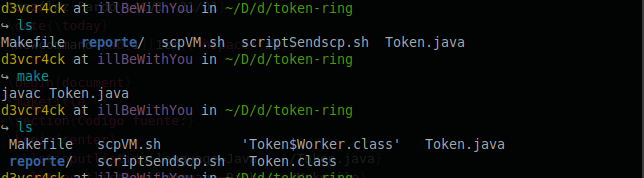
\includegraphics[scale=0.5]{img/compilacion.png}
  \\\textit{Figura 1: Compilación}
  \begin{landscape}
    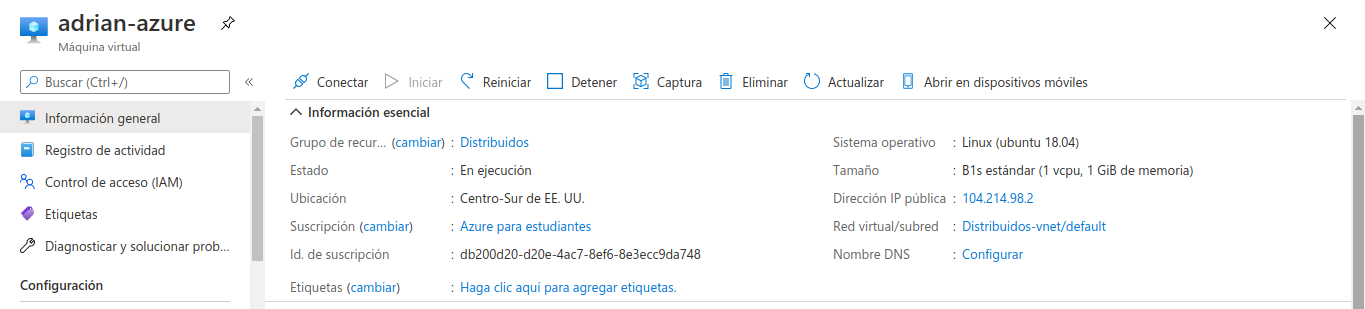
\includegraphics[scale=0.5]{img/vm-1.png}
    \\\textit{Figura 2:Maquina virtual 1 en Azure de Ubuntu Server 18}\\
    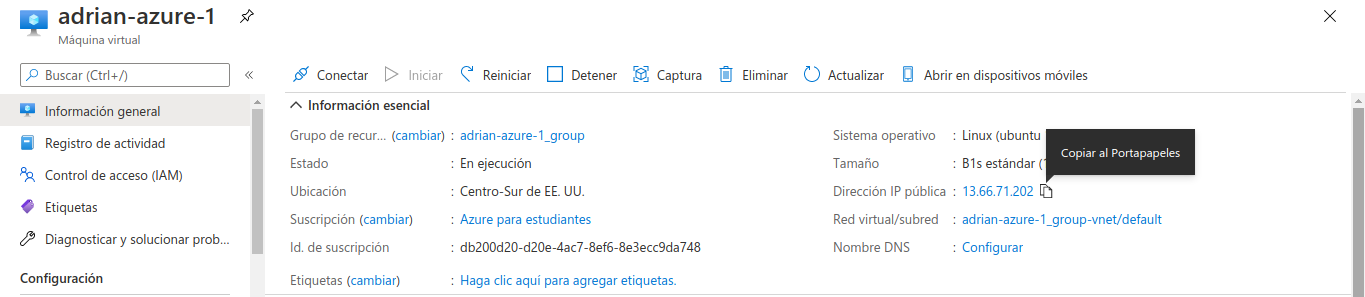
\includegraphics[scale=0.5]{img/vm-2.png}
    \\\textit{Figura 3:Maquina virtual 2 en Azure de Ubuntu Server 18}\\
    \fillandplacepagenumber
    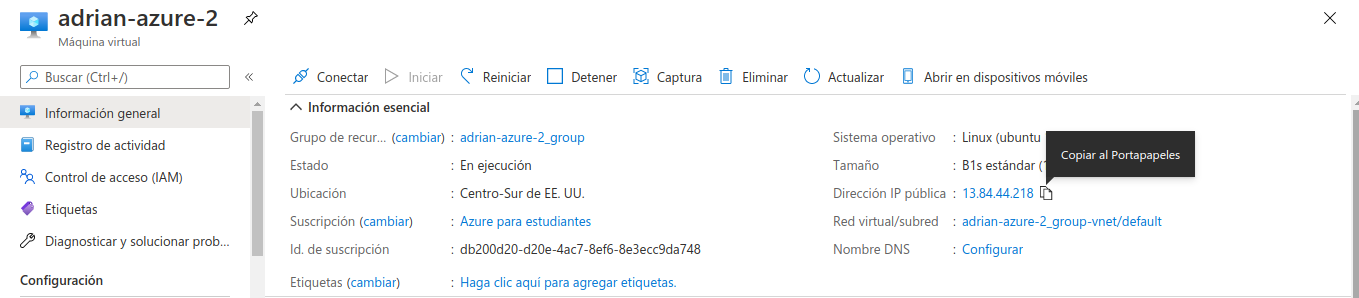
\includegraphics[scale=0.5]{img/vm-3.png}
    \\\textit{Figura 4:Maquina virtual 3 en Azure de Ubuntu Server 18}\\
    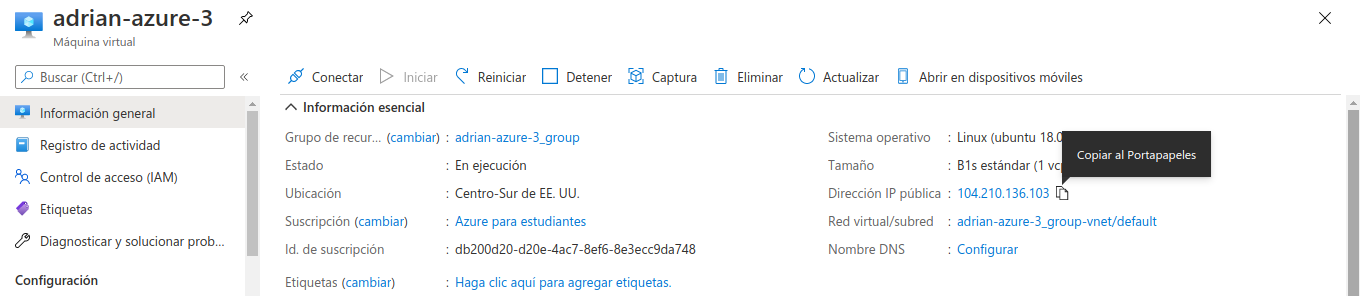
\includegraphics[scale=0.5]{img/vm-4.png}
    \\\textit{Figura 5:Maquina virtual 4 en Azure de Ubuntu Server 18}\\
    \textbf{Para las maquinas virtuales es necesario conocer las ip de las maquinas virtuales y con ello evitamos escribir muchas veces el comando scp ejecutando el siguiente script, al igual que es necesaria la instalación de los paquetes openjdk-11-jdk y cmake}
    \fillandplacepagenumber
  \end{landscape}
  \lstinputlisting[language=Bash]{../scpVM.sh}
  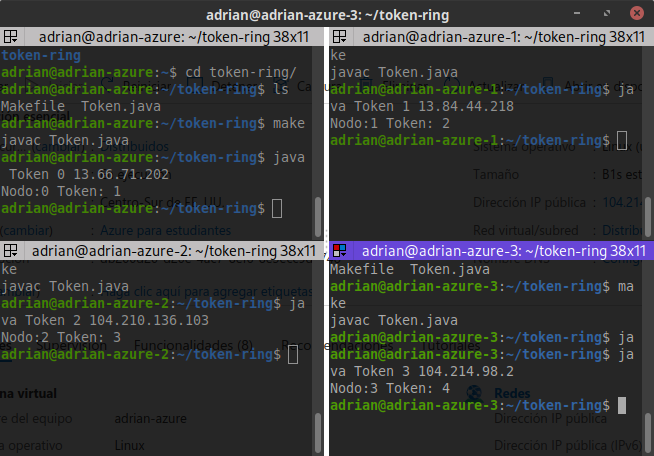
\includegraphics[scale=0.5]{img/token-azure.png}
  \\\textit{Figura 6: Muestra de la ejecución en cada VM vía ssh}\\

\end{center}
\textbf{Ahora bien en caso de querer realizar una implementación a nivel red Local con al menos 4 equipos, se puede hacer lo siguiente (destacando que ya hay un emparejamiento de llaves ssh)}\\
A nivel local se conoce la lista de los siguientes equipos:
\begin{itemize}
  \item Lenovo IP: 192.168.100.69
  \item Acer IP: 192.168.100.3
  \item Raspberry Pi 3B IP: 192.168.100.194
  \item Raspberry Pi 4B IP: 192.168.100.103
\end{itemize}
Para el cual se envio los datos con el siguiente script:
\begin{center}
  \lstinputlisting[language=Bash]{../scriptSendscp.sh}
\end{center}
Y finalmente se visualiza así:
\begin{center}
  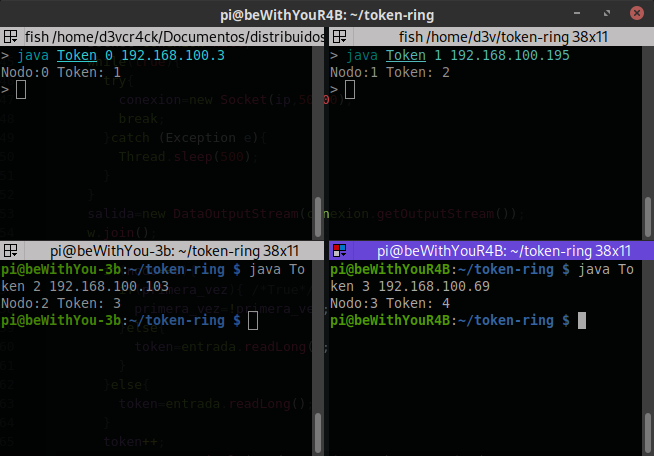
\includegraphics[scale=0.5]{img/token-2.png}
  \\\textit{Figura 7: Muestra de la ejecución en cada Nodo a nivel local vía ssh}
\end{center}
\end{document}
